\documentclass[]{tufte-handout}

% ams
\usepackage{amssymb,amsmath}

\usepackage{ifxetex,ifluatex}
\usepackage{fixltx2e} % provides \textsubscript
\ifnum 0\ifxetex 1\fi\ifluatex 1\fi=0 % if pdftex
  \usepackage[T1]{fontenc}
  \usepackage[utf8]{inputenc}
\else % if luatex or xelatex
  \makeatletter
  \@ifpackageloaded{fontspec}{}{\usepackage{fontspec}}
  \makeatother
  \defaultfontfeatures{Ligatures=TeX,Scale=MatchLowercase}
  \makeatletter
  \@ifpackageloaded{soul}{
     \renewcommand\allcapsspacing[1]{{\addfontfeature{LetterSpace=15}#1}}
     \renewcommand\smallcapsspacing[1]{{\addfontfeature{LetterSpace=10}#1}}
   }{}
  \makeatother

\fi

% graphix
\usepackage{graphicx}
\setkeys{Gin}{width=\linewidth,totalheight=\textheight,keepaspectratio}

% booktabs
\usepackage{booktabs}

% url
\usepackage{url}

% hyperref
\usepackage{hyperref}

% units.
\usepackage{units}


\setcounter{secnumdepth}{-1}

% citations
\usepackage{natbib}
\bibliographystyle{plainnat}

% pandoc syntax highlighting

% longtable
\usepackage{longtable,booktabs}

% multiplecol
\usepackage{multicol}

% strikeout
\usepackage[normalem]{ulem}

% morefloats
\usepackage{morefloats}


% tightlist macro required by pandoc >= 1.14
\providecommand{\tightlist}{%
  \setlength{\itemsep}{0pt}\setlength{\parskip}{0pt}}

% title / author / date
\title{FY19 Quarterly KPIs: Inquiries}
\author{Christine Iyer}
\date{April 23, 2019}


\begin{document}

\maketitle




\begin{center}\rule{0.5\linewidth}{\linethickness}\end{center}

\subsection{Brief Description:}\label{brief-description}

One of the KPIs we look at on a quarterly basis is \textbf{inquiries},
i.e., the number of forms completed on one of the five campaign landing
pages created for digital advertising clicks. The purpose of this report
is to look in to the recent increase in inquiries. Earlier in the year
we hypothesized that ``Gen Z'' was moving away from filling out forms;
this prompted us to consider alternative ways to engage the demographic.
However, we have noted a surge in completed forms in the past two
quarters and seek to understand more about the who is making inquiries
and when.

\begin{center}\rule{0.5\linewidth}{\linethickness}\end{center}

\subsection{Findings}\label{findings}

\textbf{Historical Inquiry Forms}

The table summarises the performance of the campaign as a whole over the
past three years.
\marginnote{Please note that the numbers for FY19 Q4 are not final. There are 2 months remaining in the quarter.}

\begin{longtable}[]{@{}lrrrr@{}}
\toprule
CampaignYR & Q1 & Q2 & Q3 & Q4\tabularnewline
\midrule
\endhead
FY17 & 119 & 82 & 139 & 107\tabularnewline
FY18 & 84 & 103 & 124 & 101\tabularnewline
FY19 & 63 & 150 & 369 & 106\tabularnewline
\bottomrule
\end{longtable}

\begin{center}\rule{0.5\linewidth}{\linethickness}\end{center}

\subsubsection{Visualization at FY
Level}\label{visualization-at-fy-level}

The following plot illustrates this quarterly historical comparison and
the recent growth in FY19.

\includegraphics{FY19_KPI_Q3_V2_files/figure-latex/unnamed-chunk-6-1}

\begin{center}\rule{0.5\linewidth}{\linethickness}\end{center}

\subsubsection{Fiscal Year Summary}\label{fiscal-year-summary}

\begin{marginfigure}
In FY17 and FY18 there were a total of 447 and 412 inquiries
respectively. This represents an overall drop of 8\%.
\end{marginfigure}

\marginnote{Please note that the numbers for FY19 Q4 are not final. There are 2 months remaining in the quarter.}

\begin{itemize}
\item
  After a relatively flat growth from FY17 to FY18 and an even more
  significant year over year drop in FY19 Q1, it appeared that we needed
  to rethink form completion as a primary message on our campaign
  landing pages.
\item
  FY19 Q2 and Q3 have shown impressive growth after a dispiriting Q1
  25\% drop from FY18
\item
  FY19 Q4 is tracking up as well and will likely surpass that of both
  FY17 and FY18.
\end{itemize}

\begin{center}\rule{0.5\linewidth}{\linethickness}\end{center}

\textbf{Campaign Level}

Since there are five distinct campaign landing pages, we need to
understand which are generating the increase inquiries. The first
cluster of plots compares the growth of each campaign side by side. Then
each campaign is shown in more detail.

\includegraphics{FY19_KPI_Q3_V2_files/figure-latex/unnamed-chunk-9-1}

\begin{center}\rule{0.5\linewidth}{\linethickness}\end{center}

\subsubsection{Undergraduate Inquiries}\label{undergraduate-inquiries}

\begin{longtable}[]{@{}llrrrr@{}}
\toprule
Campaign & FY & Q1 & Q2 & Q3 & Q4\tabularnewline
\midrule
\endhead
UG & FY17 & 78 & 45 & 91 & 68\tabularnewline
UG & FY18 & 36 & 51 & 65 & 53\tabularnewline
UG & FY19 & 29 & 52 & 154 & 52\tabularnewline
\bottomrule
\end{longtable}

\includegraphics{FY19_KPI_Q3_V2_files/figure-latex/unnamed-chunk-10-1}

\subsubsection{Transfer Inquiries}\label{transfer-inquiries}

\begin{longtable}[]{@{}llrrrr@{}}
\toprule
Campaign & FY & Q1 & Q2 & Q3 & Q4\tabularnewline
\midrule
\endhead
TR & FY17 & 27 & 18 & 21 & 23\tabularnewline
TR & FY18 & 27 & 32 & 31 & 25\tabularnewline
TR & FY19 & 14 & 35 & 86 & 18\tabularnewline
\bottomrule
\end{longtable}

\includegraphics{FY19_KPI_Q3_V2_files/figure-latex/unnamed-chunk-11-1}

\subsubsection{Graduate Inquiries}\label{graduate-inquiries}

\begin{longtable}[]{@{}llrrrr@{}}
\toprule
Campaign & FY & Q1 & Q2 & Q3 & Q4\tabularnewline
\midrule
\endhead
GR & FY17 & 10 & 12 & 13 & 12\tabularnewline
GR & FY18 & 12 & 13 & 9 & 12\tabularnewline
GR & FY19 & 13 & 33 & 85 & 21\tabularnewline
\bottomrule
\end{longtable}

\includegraphics{FY19_KPI_Q3_V2_files/figure-latex/unnamed-chunk-12-1}

\subsubsection{Degree Completion
Inquiries}\label{degree-completion-inquiries}

\begin{longtable}[]{@{}llrrrr@{}}
\toprule
Campaign & FY & Q1 & Q2 & Q3 & Q4\tabularnewline
\midrule
\endhead
DC & FY17 & 1 & 1 & 1 & NA\tabularnewline
DC & FY18 & 2 & NA & 15 & 2\tabularnewline
DC & FY19 & 2 & 8 & 10 & 1\tabularnewline
\bottomrule
\end{longtable}

\includegraphics{FY19_KPI_Q3_V2_files/figure-latex/unnamed-chunk-13-1}

\subsubsection{Online Program Inquiries}\label{online-program-inquiries}

\begin{longtable}[]{@{}llrrrr@{}}
\toprule
Campaign & FY & Q1 & Q2 & Q3 & Q4\tabularnewline
\midrule
\endhead
OL & FY17 & 3 & 6 & 13 & 4\tabularnewline
OL & FY18 & 7 & 7 & 4 & 9\tabularnewline
OL & FY19 & 5 & 22 & 34 & 14\tabularnewline
\bottomrule
\end{longtable}

\includegraphics{FY19_KPI_Q3_V2_files/figure-latex/unnamed-chunk-14-1}

\begin{center}\rule{0.5\linewidth}{\linethickness}\end{center}

\textbf{Campaign Results Summary}

\begin{itemize}
\item
  We see growth across all campaigns, with the exception of the degree
  completion program.
\item
  Graduate and Transfer campaigns have shown new inquiry activity,
  outside of the regualr seasonal pattern, in the beginning late
  November.
\item
  FY19 Graduate ads were more varied.
\item
  FY19 Transfer ads
\item
  Younger students are still filling out inquiries judging from the last
  several months.
\item
  There is an obvious interest in online degree programs at USM.
\end{itemize}

\begin{center}\rule{0.5\linewidth}{\linethickness}\end{center}

\textbf{Inquiries by month and program}

Inquiries for both undergraduate and graduate degree programs begin to
pick up in December and remain steady throughout the spring. Judging
from historical performance, inquiries taper during the final quarter of
the fiscal year. Inquiries from potential transfer students have
recently peaked in the winter months, perhaps at the end of the fall
semester.

The cluster of plots below illustrate a comparison of monthly patterns
over the past three years.

\includegraphics{FY19_KPI_Q3_V2_files/figure-latex/unnamed-chunk-16-1}

\textbf{Location}

It would be helpful to know where geographically these inquiries are
coming from. Between 1/3 and 1/2 of the inquiries are from an unknown
geographic origin, we can only make general, but useful observations,
comparing the shift in inquiries from in-state, out-of-state, and
unknown origin.

The cluster of plots below represents the breakdown of where inquiries
are coming from by percent and program. We see in FY19 that a much
larger percentage of inquiries to the Undergraduate program the
out-of-state HS students, shown in red.

\includegraphics{FY19_KPI_Q3_V2_files/figure-latex/unnamed-chunk-17-1}

\begin{center}\rule{0.5\linewidth}{\linethickness}\end{center}

\subsection{Inquiry Sources}\label{inquiry-sources}

\begin{figure}
\centering
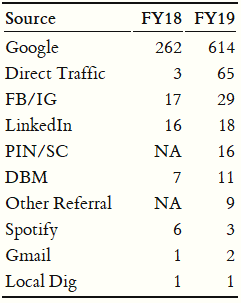
\includegraphics{Capture.PNG}
\caption{}
\end{figure}

\begin{center}\rule{0.5\linewidth}{\linethickness}\end{center}

\subsection{Conclusion}\label{conclusion}

\begin{itemize}
\item
  While there is a narrower window for transfer inquiries, inquiries for
  both graduate and undergraduate programs begin to pick up in December.
\item
  As we know, they slow in the summer and remain so until December,
  except for those inquiring about the degree completion programs.
\item
  However, it is probably still wise to consider alternative ways to
  reach all demographics. \textbf{Notes}
\end{itemize}

\bibliography{skeleton.bib}



\end{document}
